% Questions on PDF page 134
\documentclass[11pt]{article}

\usepackage[utf8]{inputenc}
\usepackage[a4paper, margin=1in]{geometry}
\usepackage{booktabs}
\usepackage{enumerate}
\usepackage{physics}
\usepackage{amsmath}
\usepackage{amsfonts}
\usepackage{graphicx}
\usepackage{siunitx}
\usepackage{textcomp}
\usepackage{hyperref}

\bibliographystyle{ieeetr}
\graphicspath{{./figures}}

\title{Big Data (AES 630) Homework 2}
\author{Mitchell Dodson}
\date{February 8, 2024}

\newcommand*{\problem}[2]{
    \begin{table}[ht]
    \centering
        \begin{tabular}{ | p{.1\linewidth} p{.9\linewidth} | }
            \hline
            \vspace{.3em}\textbf{\large#1:} & \vspace{.3em}\small{#2}\hspace{.2em}\vspace{.5em} \\ \hline
        \end{tabular}
    \end{table}
}

\begin{document}

\noindent
{\Large\textbf{Big Data (AES 690) Homework 2}}

\noindent
\large{Mitchell Dodson}

\noindent
\large{February 8, 2024}

\section{Data compression}

The dataset I will use for this assignment is an 8-dimensional lookup table for spectral flux. The table has axes for atmosphere profile, cloud height, cloud optical depth, cloud particle size, solar zenith, wavelength, height, and flux type, and has dimensional shape:

\begin{center}
    (6, 4, 2, 25, 8, 241, 33, 4)
\end{center}

I chose to use the lookup table out of curiosity for how the compression would respond to the table's high dimensionality and redundancy across some axes. The table was generated using a generalized python wrapper I made for the SBDART radiative transfer model, which is available on my github: \url{https://github.com/Mitchell-D/quickrad}

\begin{equation}
    (6 \cdot 4 \cdot 2 \cdot 25  \cdot 8 \cdot 241 \cdot 33 \cdot 4) \cdot 8\,\si{B} = \num{2.4431616e9}\,\si{B}
\end{equation}

Multiplying the dimensions together and scaling by 8 bytes (since SBDART produces float64 values), we find that the size of the data cube alone is 2,443,161,600 bytes. In practice, however, the stored netCDF file is 2,443,177,101 bytes, which is 15,501 bytes more. This is because the full netCDF file also contains file structure data, labels, and coordinate arrays.

\begin{figure}[h!]
    \centering

    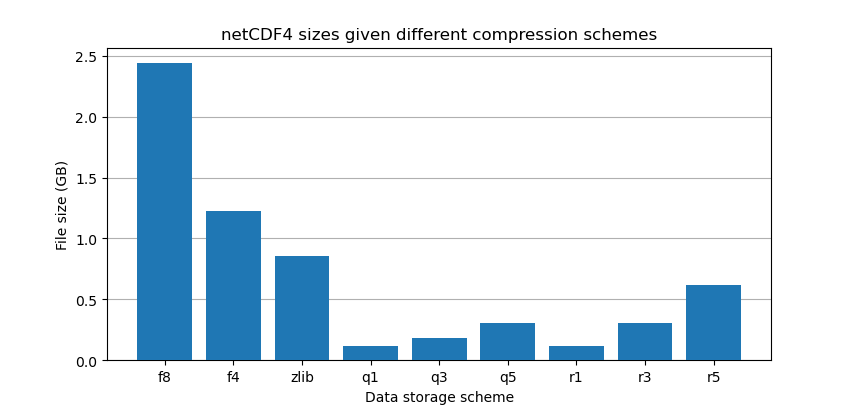
\includegraphics[width=.7\paperwidth]{figs/sizes.png}

    \caption{File sizes after data reduction. `f4' and `f8' represent 32-bit and 64-bit floats, respectively, r1-r5 represents 64 bit float values rounded to the 1st-5th decimals, and q1-q5 represents 64 bit float values quantized to the 1st-5th significant digits with BitGroom. Each quantized and rounded file is compressed using zlib.}
    \label{sizes}
\end{figure}

\begin{table}[h!]
    \centering
    \begin{tabular}{c | c c c c c c c c}
        & float32 & float64 + zlib & quant 1 & quant 3 & quant 5 & round 1 & round 3 & round 5 \\
        \hline
        ratio & 2.000 & 2.847 & 21.020 & 13.571 & 7.923 & 21.038 & 7.925 & 3.977 \\
        error & 5.47e-8 & 0 & 3.03e-2 & 5.30e-4 & 4.09e-6 & 1.87e-2 & 1.04e-4 & 1.71e-7 \\
    \end{tabular}
    \caption{zlib compression ratio and error amount for size reduction, quantization, and rounding.}
    \label{ratios}
\end{table}

Figure \ref{sizes} and Table \ref{ratios} show the file sizes and compression ratios of the dataset after compression by data type reduction, value rounding, and significant digit quantization. These results show that compression with zlib reduces the float64 file size by about 2.847 times; even more than data type reduction to float32, which reduces the size to almost exactly half. Rounding and quantization to between 1 and 5 decimals or significant digits was even more effective, with compression ratios greater than 21.


\begin{figure}[h!]
    \centering
    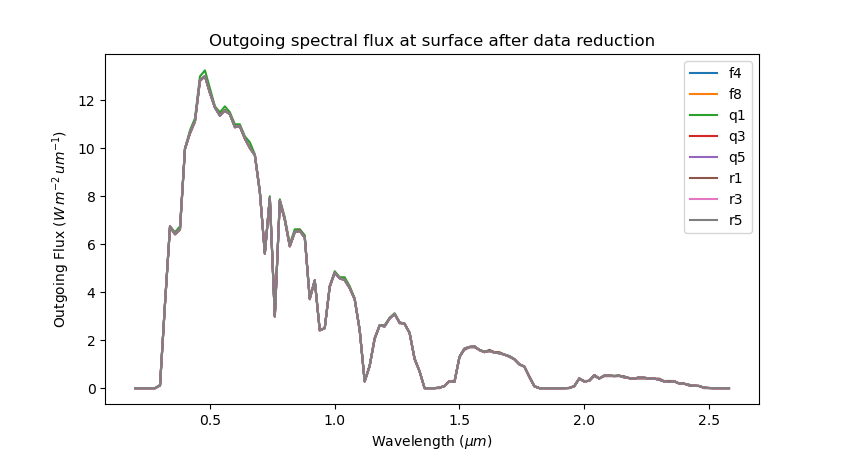
\includegraphics[width=.75\paperwidth]{figs/sflux.png}

    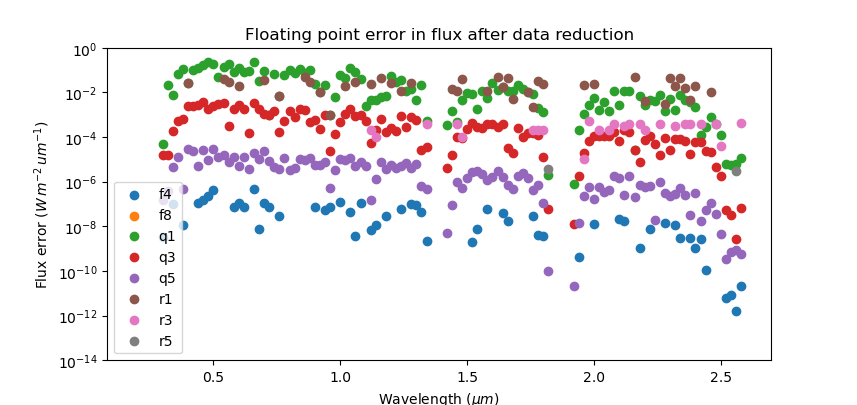
\includegraphics[width=.75\paperwidth]{figs/error2.png}
    \caption{Outgoing radiative flux at the surface wrt wavelength, and floating point error rate wrt wavelength given each of the compression schemes. Data are extracted by assuming outgoing flux measurements were taken at the surface at noon with a tropical atmosphere, and a water cloud at $1\,\si{km}$ having optical depth $\tau=0.01$ and effective particle size $r=10\,\si{\mu m}$.}
    \label{sflux}
\end{figure}

The first image in Figure \ref{sflux} shows the spectral distribution of reflected solar flux after the data was subjected to multiple data compression measures. The data loss isn't immediately apparent at this scale, except for some variation in the 1-digit quantized curve near the peak values. The second image in Figure \ref{sflux} displays the magnitude of floating point error on a log scale. The different methods have error magnitudes that form discrete levels depending on their precision, and corresponding closely to the magnitude of file size reduction. This makes apparent the impact of lossy compression on data quality. Many values had zero error in each compression method, which is unsurprising since regardless of precision, all floats are ultimately discretized to values governed by their exponent and mantissa bits.

\section{Cloud data access}

\begin{figure}[h!]
    \centering
    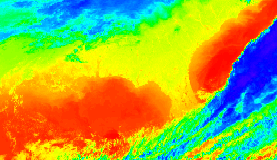
\includegraphics[width=.3\linewidth]{figs/goes_0.png}
    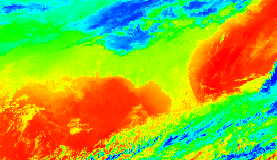
\includegraphics[width=.3\linewidth]{figs/goes_4.png}
    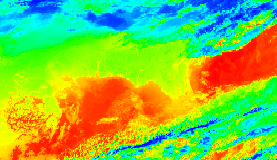
\includegraphics[width=.3\linewidth]{figs/goes_8.png}

    \vspace{.25em}

    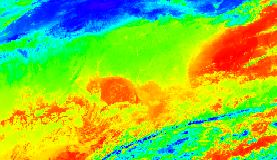
\includegraphics[width=.3\linewidth]{figs/goes_12.png}
    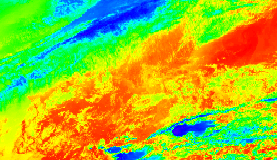
\includegraphics[width=.3\linewidth]{figs/goes_16.png}
    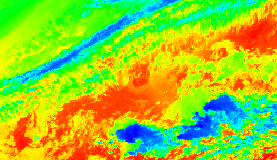
\includegraphics[width=.3\linewidth]{figs/goes_20.png}

    \vspace{.25em}

    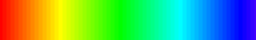
\includegraphics[width=.4\linewidth]{figs/cbar.png}

    \caption{GMGSI longwave GOES imagery over SEUS, every 4 hours starting at 0Z on Jan 15, 2024, showing the gradual formation of a warm stratiform cloud deck from the Gulf of Mexico. Further into the continent, low clouds from a frigid airmass dominate the scene.}
\end{figure}

The version of GMGSI data hosted on the AWS bucket is stored as integers in the range $[0,255]$. I used s3fs and \texttt{xarray.open\_mfdataset} to load all the hourly files from the UTC day of January 15, 2024, then restricted the domain to only include SEUS pixels using boolean masks derived from the thresholds $lat \in [25,35]$ and $lon \in [-95,-75]$.

I wasn't able to find any documentation of the bounds used for normalizing the GMGSI imagery, but the mean value is 116.243, or 0.45585 if normalized to [0,1].

\vspace{1em}
\centering\large
\textbf{All of my code for this assignment is available on github at:}

\centering\large
\url{https://github.com/Mitchell-D/aes690hw2}

\end{document}

\begin{figure}[h!]\label{q1q2}
    \centering
    \begin{tabular}{ c c c | c}
    \end{tabular}
\end{figure}

